%<*mtag1>
\begin{figure}[H]
\centering
\captionsetup{width=.8\linewidth}
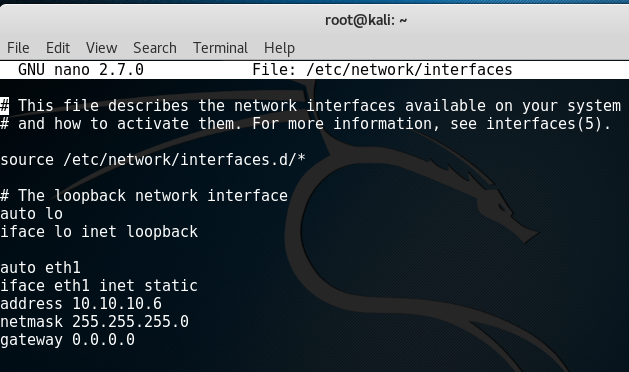
\includegraphics[scale=0.5]{img/Ex4_1.png}
\caption{Setting a static IP on Kali Linux VM}
\label{fig:kaliip}
\centering
\end{figure}
%</mtag1>

%<*mtag2>
\begin{figure}[H]
\centering
\captionsetup{width=.8\linewidth}
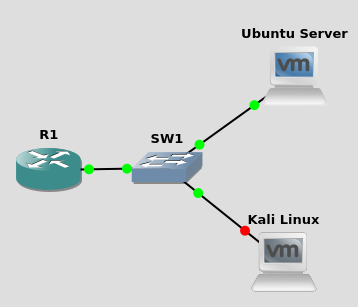
\includegraphics[scale=0.5]{img/Ex4_2.png}
\caption{GNS3 topology of Exercise 4}
\label{fig:ex4setup}
\centering
\end{figure}
%</mtag2>

%<*mtag3>
\begin{figure}[H]
\centering
\captionsetup{width=.8\linewidth}
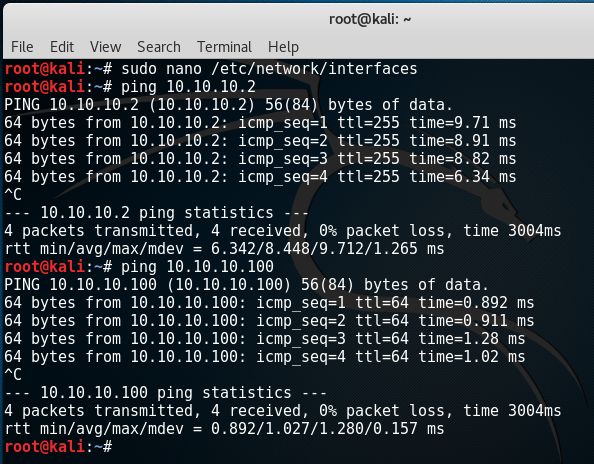
\includegraphics[scale=0.5]{img/Ex4_3.png}
\caption{Issue of pings to the TACACS+ router (10.10.10.2) and the TACACS+ server (10.10.10.100) from Kali Linux VM}
\label{fig:pinging}
\centering
\end{figure}
%</mtag3>

%<*mtag4>
\begin{figure}[H]
\centering
\captionsetup{width=.8\linewidth}
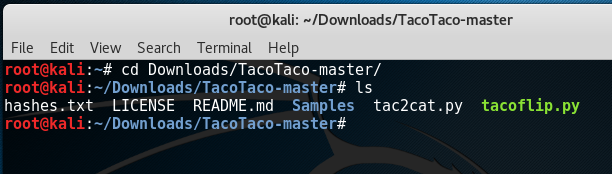
\includegraphics[scale=0.5]{img/Ex4_4.png}
\caption{Shows the extracted TacoTaco project to the Downloads folder in Kali}
\label{fig:tacoproof}
\centering
\end{figure}
%</mtag4>

%<*mtag5>
\begin{figure}[H]
\centering
\captionsetup{width=.8\linewidth}
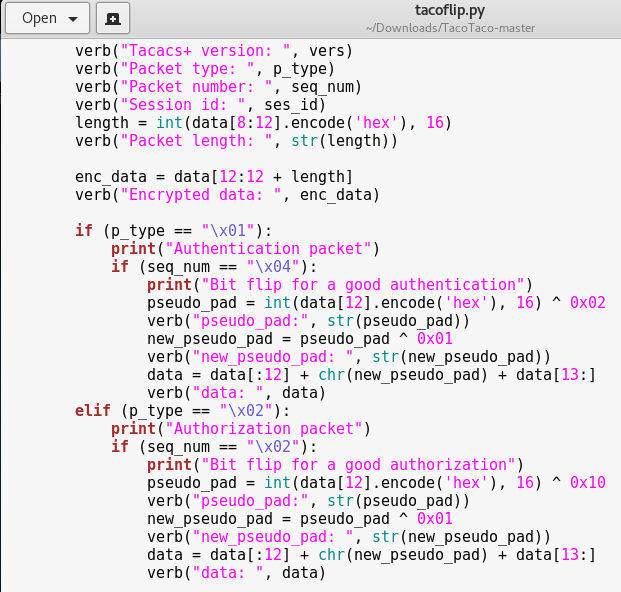
\includegraphics[scale=0.5]{img/Ex4_5.png}
\caption{Part of the expansion of the tacoflip.py file in gedit. Here you can see the process of how the script carries out the bitflipping attack as explained in Question 3.}
\label{fig:tacoflip}
\centering
\end{figure}
%</mtag5>

%<*mtag6>
\begin{figure}[H]
\centering
\captionsetup{width=.8\linewidth}
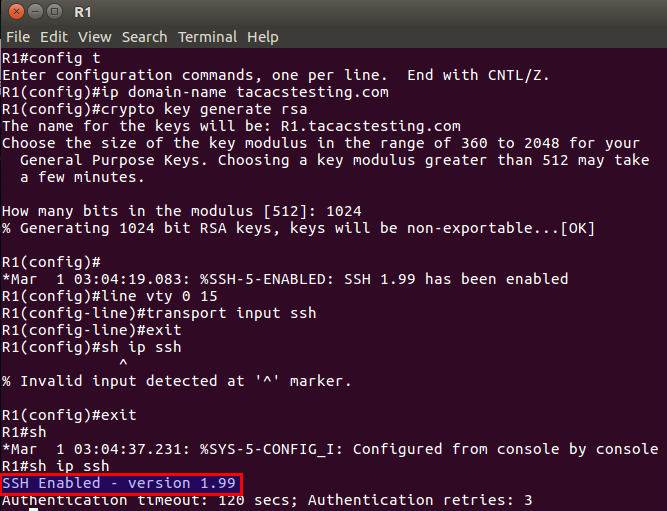
\includegraphics[scale=0.5]{img/Ex4_6.png}
\caption{Setting up SSH in the console of the cisco router. Here, you can see that the version is 1.99, and that the keys were generated under the created domain name of "tacacstesting.com"}
\label{fig:ex4ssh}
\centering
\end{figure}
%</mtag6>

%<*mtag7>
\begin{figure}[H]
\centering
\captionsetup{width=.8\linewidth}
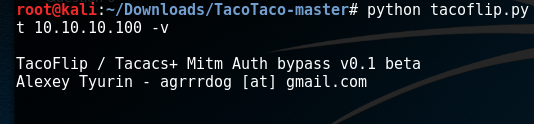
\includegraphics[scale=0.5]{img/Selection_070.png}
\caption{Output of running the tacoflip.py file initially.}
\label{fig:1sttaco}
\centering
\end{figure}
%</mtag7>

%<*mtag8>
\begin{figure}[H]
\centering
\captionsetup{width=.8\linewidth}
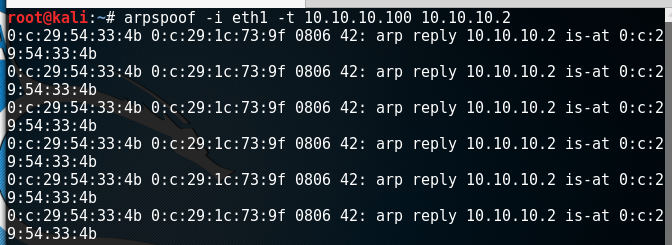
\includegraphics[scale=0.5]{img/Ex4_7.png}
\caption{Shows the arp poisoning of the TACACS+ server and TACACS+ router. There is also another instance of this attack in another terminal, not shown (swapping the ip address order).}
\label{fig:arpspoof}
\centering
\end{figure}
%</mtag8>

%<*mtag9>
\begin{figure}[H]
\centering
\captionsetup{width=.8\linewidth}
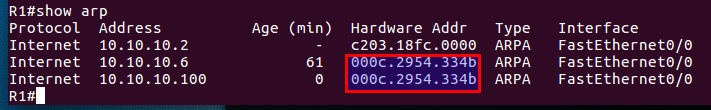
\includegraphics[scale=0.5]{img/Ex4_8.png}
\caption{Proof that the arpspoof command was successful. In this figure, you can see that the attacker (10.10.10.6) has the same hardware or MAC address as the TACACS+ server (10.10.10.100). This shared address is \texttt{000c.2954.334b}.}
\label{fig:showarp}
\centering
\end{figure}
%</mtag9>

%<*mtag10>
\begin{figure}[H]
\centering
\captionsetup{width=.8\linewidth}
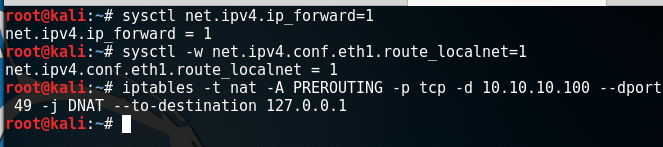
\includegraphics[scale=0.5]{img/Ex4_9.png}
\caption{Shows the sysctl and iptables commands.}
\label{fig:3commands}
\centering
\end{figure}
%</mtag10>

%<*mtag11>
\begin{figure}[H]
\centering
\captionsetup{width=.8\linewidth}
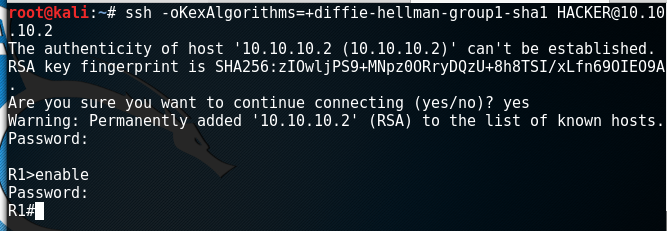
\includegraphics[scale=0.5]{img/Ex4_11.png}
\caption{Shows the attacker ssh-ing to the TACACS+ router with invalid credentials with the aid of the tacoflip.py file.}
\label{fig:hahassh}
\centering
\end{figure}
%</mtag11>

%<*mtag12>
\begin{figure}[H]
\centering
\captionsetup{width=.8\linewidth}
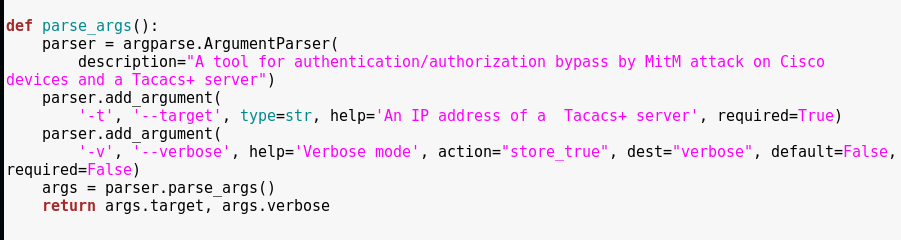
\includegraphics[scale=0.5]{img/Selection_071.png}
\caption{Shows the beginning of the expansion of the tacoflip.py file, showing the available options.}
\label{fig:tacooptions}
\centering
\end{figure}
%</mtag12>

%<*mtag13>
\begin{figure}[H]
\centering
\captionsetup{width=.8\linewidth}
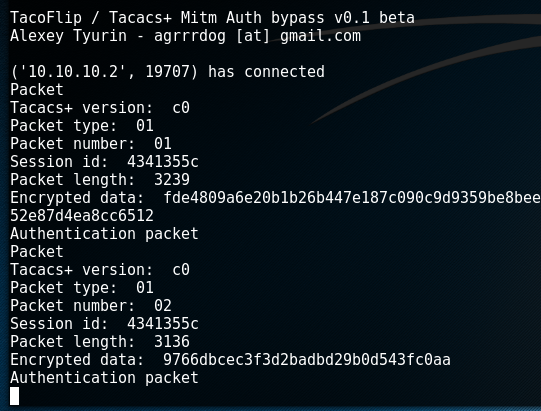
\includegraphics[scale=0.5]{img/Ex4_10.png}
\caption{Shows the initial output of the tacoflip.py file when the attacker issues the first ssh command to login.}
\label{fig:tacoflip1}
\centering
\end{figure}
%</mtag13>

%<*mtag14>
\begin{figure}[H]
\centering
\captionsetup{width=.8\linewidth}
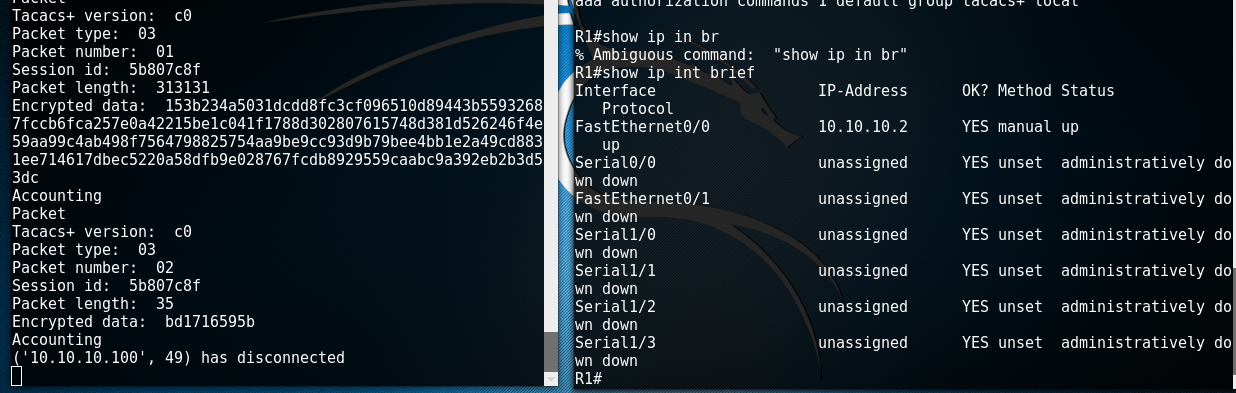
\includegraphics[scale=0.5]{img/Ex4_12.png}
\caption{Issue of \texttt{show ip int brief} to see the available interfaces on the router, while logged in with the TacoTaco attack. Also in this figure, you can see the output of the tacoflip.py file}
\label{fig:showipkali}
\centering
\end{figure}
%</mtag14>

%<*mtag15>
\begin{figure}[H]
\centering
\captionsetup{width=.8\linewidth}
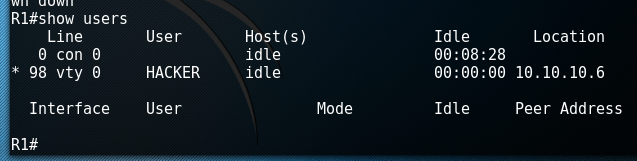
\includegraphics[scale=0.5]{img/Ex4_13.png}
\caption{Issue of \texttt{show users} to see the currently logged in users while loggin in with the TacoTaco attack. Here you can see the user with invalid credentials logged in, and the address of where it is located.}
\label{fig:showuserskali}
\centering
\end{figure}
%</mtag15>

%<*mtag16>
\begin{figure}[H]
\centering
\captionsetup{width=.8\linewidth}
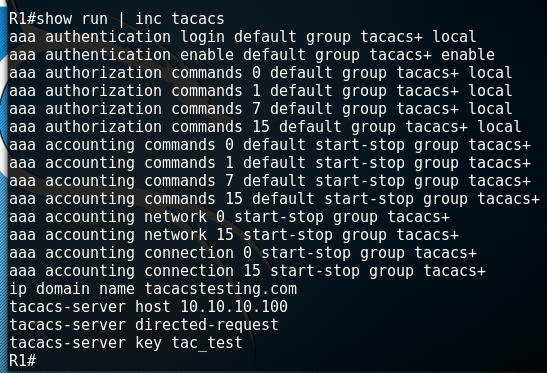
\includegraphics[scale=0.5]{img/Ex4_14.png}
\caption{Issue of the \texttt{show run \text{\textbar} inc tacacs} command while logged in with the TacoTaco attack. Here we use the "\text{\textbar} inc tacacs" to only show the running configuration associated with the TACACS+ protocol.}
\label{fig:showrunkali}
\centering
\end{figure}
%</mtag16>

%<*mtag17>
\begin{figure}[H]
\centering
\captionsetup{width=.8\linewidth}
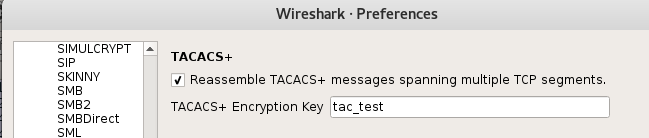
\includegraphics[scale=0.5]{img/Ex4_15.png}
\caption{Edit - Preferences - Protocols - TACACS+}
\label{fig:wiresharkkey}
\centering
\end{figure}
%</mtag17>

%<*mtag18>
\begin{figure}[H]
\centering
\captionsetup{width=.8\linewidth}
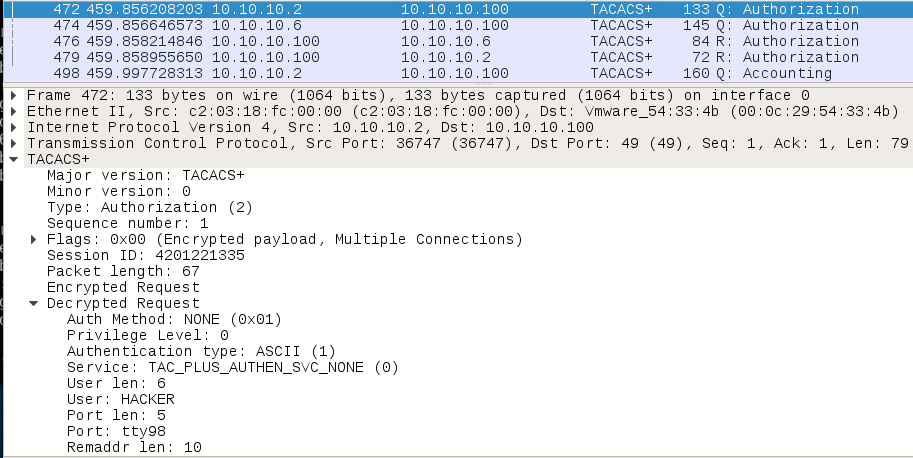
\includegraphics[scale=0.5]{img/Ex4_16.png}
\caption{Decrypted Authorization packet. Here you can see the user name of the user who logged in, the privilege level that the user has, and more all in plain-text.}
\label{fig:authpacket1}
\centering
\end{figure}
%</mtag18>

%<*mtag19>
\begin{figure}[H]
\centering
\captionsetup{width=.8\linewidth}
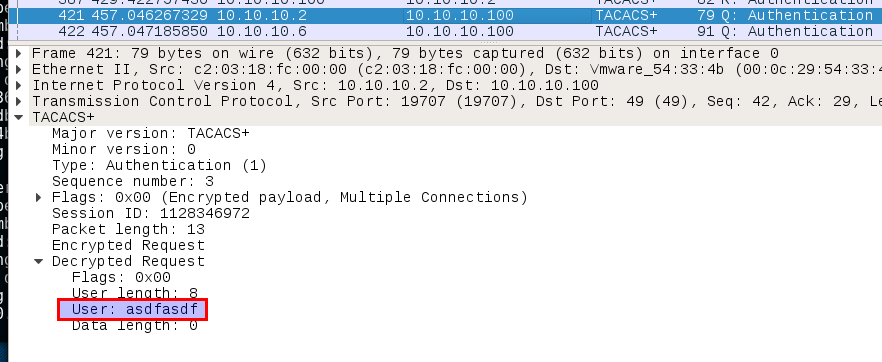
\includegraphics[scale=0.5]{img/Ex4_17.png}
\caption{Decrypted Authentication packet. Here you can see the password that the user (attacker) inputted when the tacoflip.py attack was used.}
\label{fig:authpacket2}
\centering
\end{figure}
%</mtag19>

%<*mtag20>
\begin{figure}[H]
\centering
\captionsetup{width=.8\linewidth}
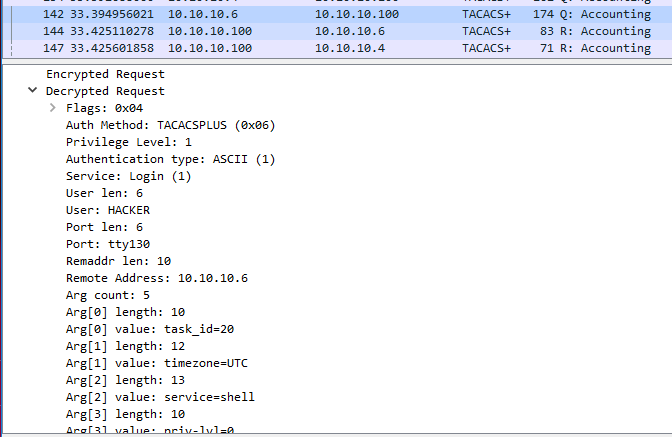
\includegraphics[scale=0.8]{img/Capture.PNG}
\caption{Decrypted Accounting packet. Here you can see auth method, username, remote address, the commands that the user inputted, and much more in plain-text.}
\label{fig:accpacket}
\centering
\end{figure}
%</mtag20>

%<*mtag21>
\begin{figure}[H]
\centering
\captionsetup{width=.8\linewidth}
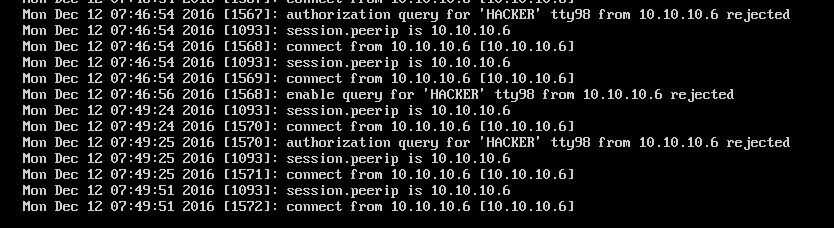
\includegraphics[scale=0.5]{img/Ex4_18.png}
\caption{tac\textunderscore plus.log}
\label{fig:tacpluslog}
\centering
\end{figure}
%</mtag21>

%<*mtag22>
\begin{figure}[H]
\centering
\captionsetup{width=.8\linewidth}
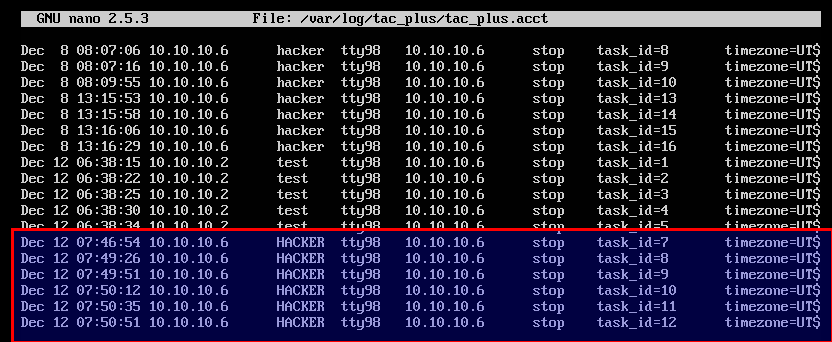
\includegraphics[scale=0.5]{img/Ex4_19.png}
\caption{tac\textunderscore plus.acct}
\label{fig:tacccount}
\centering
\end{figure}
%</mtag22>

%<*mtag23>
\begin{figure}[H]
\centering
\captionsetup{width=.8\linewidth}
\includegraphics[scale=0.5]{img/Ex1S0_1.png}
\caption{}
\label{fig:}
\centering
\end{figure}
%</mtag23>

%<*mtag24>
\begin{figure}[H]
\centering
\captionsetup{width=.8\linewidth}
\includegraphics[scale=0.5]{img/Ex1S0_1.png}
\caption{}
\label{fig:}
\centering
\end{figure}
%</mtag24>

%<*mtag25>
\begin{figure}[H]
\centering
\captionsetup{width=.8\linewidth}
\includegraphics[scale=0.5]{img/Ex1S0_1.png}
\caption{}
\label{fig:}
\centering
\end{figure}
%</mtag25>

%<*mtag26>
\begin{figure}[H]
\centering
\captionsetup{width=.8\linewidth}
\includegraphics[scale=0.5]{img/Ex1S0_1.png}
\caption{}
\label{fig:}
\centering
\end{figure}
%</mtag26>

%<*mtag27>
\begin{figure}[H]
\centering
\captionsetup{width=.8\linewidth}
\includegraphics[scale=0.5]{img/Ex1S0_1.png}
\caption{}
\label{fig:}
\centering
\end{figure}
%</mtag27>

%<*mtag28>
\begin{figure}[H]
\centering
\captionsetup{width=.8\linewidth}
\includegraphics[scale=0.5]{img/Ex1S0_1.png}
\caption{}
\label{fig:}
\centering
\end{figure}
%</mtag28>

%<*mtag29>
\begin{figure}[H]
\centering
\captionsetup{width=.8\linewidth}
\includegraphics[scale=0.5]{img/Ex1S0_1.png}
\caption{}
\label{fig:}
\centering
\end{figure}
%</mtag29>

%<*mtag30>
\begin{figure}[H]
\centering
\captionsetup{width=.8\linewidth}
\includegraphics[scale=0.5]{img/Ex1S0_1.png}
\caption{}
\label{fig:}
\centering
\end{figure}
%</mtag30>

%<*mtag31>
\begin{figure}[H]
\centering
\captionsetup{width=.8\linewidth}
\includegraphics[scale=0.5]{img/Ex1S0_1.png}
\caption{}
\label{fig:}
\centering
\end{figure}
%</mtag31>

%<*mtag32>
\begin{figure}[H]
\centering
\captionsetup{width=.8\linewidth}
\includegraphics[scale=0.5]{img/Ex1S0_1.png}
\caption{}
\label{fig:}
\centering
\end{figure}
%</mtag32>

%<*mtag33>
\begin{figure}[H]
\centering
\captionsetup{width=.8\linewidth}
\includegraphics[scale=0.5]{img/Ex1S0_1.png}
\caption{}
\label{fig:}
\centering
\end{figure}
%</mtag33>

%<*mtag34>
\begin{figure}[H]
\centering
\captionsetup{width=.8\linewidth}
\includegraphics[scale=0.5]{img/Ex1S0_1.png}
\caption{}
\label{fig:}
\centering
\end{figure}
%</mtag34>

%<*mtag35>
\begin{figure}[H]
\centering
\captionsetup{width=.8\linewidth}
\includegraphics[scale=0.5]{img/Ex1S0_1.png}
\caption{}
\label{fig:}
\centering
\end{figure}
%</mtag35>

%<*mtag36>
\begin{figure}[H]
\centering
\captionsetup{width=.8\linewidth}
\includegraphics[scale=0.5]{img/Ex1S0_1.png}
\caption{}
\label{fig:}
\centering
\end{figure}
%</mtag36>

%<*mtag37>
\begin{figure}[H]
\centering
\captionsetup{width=.8\linewidth}
\includegraphics[scale=0.5]{img/Ex1S0_1.png}
\caption{}
\label{fig:}
\centering
\end{figure}
%</mtag37>

%<*mtag1>
\begin{figure}[H]
\centering
\captionsetup{width=.8\linewidth}
\includegraphics[scale=0.5]{img/Ex1S0_1.png}
\caption{}
\label{fig:}
\centering
\end{figure}
%</mtag38>

%<*mtag39>
\begin{figure}[H]
\centering
\captionsetup{width=.8\linewidth}
\includegraphics[scale=0.5]{img/Ex1S0_1.png}
\caption{}
\label{fig:}
\centering
\end{figure}
%</mtag39>

%<*mtag40>
\begin{figure}[H]
\centering
\captionsetup{width=.8\linewidth}
\includegraphics[scale=0.5]{img/Ex1S0_1.png}
\caption{}
\label{fig:}
\centering
\end{figure}
%</mtag40>

%<*mtag42>
\begin{figure}[H]
\centering
\captionsetup{width=.8\linewidth}
\includegraphics[scale=0.5]{img/Ex1S0_1.png}
\caption{}
\label{fig:}
\centering
\end{figure}
%</mtag41>

%<*mtag43>
\begin{figure}[H]
\centering
\captionsetup{width=.8\linewidth}
\includegraphics[scale=0.5]{img/Ex1S0_1.png}
\caption{}
\label{fig:}
\centering
\end{figure}
%</mtag43>

%<*mtag44>
\begin{figure}[H]
\centering
\captionsetup{width=.8\linewidth}
\includegraphics[scale=0.5]{img/Ex1S0_1.png}
\caption{}
\label{fig:}
\centering
\end{figure}
%</mtag44>

%<*mtag45>
\begin{figure}[H]
\centering
\captionsetup{width=.8\linewidth}
\includegraphics[scale=0.5]{img/Ex1S0_1.png}
\caption{}
\label{fig:}
\centering
\end{figure}
%</mtag45>

%<*mtag46>
\begin{figure}[H]
\centering
\captionsetup{width=.8\linewidth}
\includegraphics[scale=0.5]{img/Ex1S0_1.png}
\caption{}
\label{fig:}
\centering
\end{figure}
%</mtag46>

%<*mtag47>
\begin{figure}[H]
\centering
\captionsetup{width=.8\linewidth}
\includegraphics[scale=0.5]{img/Ex1S0_1.png}
\caption{}
\label{fig:}
\centering
\end{figure}
%</mtag47>

%<*mtag48>
\begin{figure}[H]
\centering
\captionsetup{width=.8\linewidth}
\includegraphics[scale=0.5]{img/Ex1S0_1.png}
\caption{}
\label{fig:}
\centering
\end{figure}
%</mtag48>

%<*mtag49>
\begin{figure}[H]
\centering
\captionsetup{width=.8\linewidth}
\includegraphics[scale=0.5]{img/Ex1S0_1.png}
\caption{}
\label{fig:}
\centering
\end{figure}
%</mtag49>

%<*mtag50>
\begin{figure}[H]
\centering
\captionsetup{width=.8\linewidth}
\includegraphics[scale=0.5]{img/Ex1S0_1.png}
\caption{}
\label{fig:}
\centering
\end{figure}
%</mtag50>